
In this section we will use \mRa-estimators for some specific families of probability distributions. As was stated above, results for normal model were already presented in  \cite{Vajda2009}, \cite{Demut2010}. Therefore we focused on exponential, Laplace, Cauchy and Weibull families. In case of these families we focused on deriving specific simple forms of estimator according to \eqref{eq:renEstimator} and also the form of influence function \eqref{eq:IF}.

\subsection{Laplace distribution} 
Here we use \mRa-estimators to estimate parameter $\theta = (\mu,\lambda)$ in Laplace model. Laplace probability density function can be written as 
\begin{equation}
	p_\theta = \frac{1}{2\lambda} e^{-\frac{|x-\mu|}{\lambda}}, \qquad \mu\in \mathbb{R},\, \lambda>0.
\end{equation}
For $\alpha = 0$ is the estimator \eqref{eq:renEstimator} equal to maximum likelihood estimator
\begin{align}
	\hat{\theta}_{\mathfrak{R}_0,n} & = \arg \max_{\theta \in \Theta} \frac{1}{n} \sum^n_{i=1} \ln \left[ \frac{1}{2\lambda}\exp \left[-\frac{|x_i-\mu|}{\lambda} \right] \right] \nonumber \\
	& =  \arg \max_{\theta \in \Theta} \left[ \ln \frac{1}{2\lambda} - \frac{1}{n} \sum^n_{i=1} \frac{|x_i-\mu|}{\lambda} \right].
\end{align}
Condition \ref{eq:betaCond} holds for all $\beta>0$, therefore we can \mRa-estimator \eqref{eq:renEstimator} of parameters of Laplace distribution write for $\alpha>0$ as
\begin{equation}
	\hat{\theta}_{\mathfrak{R}_\alpha,n} = \arg \max_{\theta \in \Theta} \left[ (2\lambda)^{-\frac{\alpha}{1+\alpha}} \frac{1}{n} \sum_{i=1}^n \exp \left[-\alpha\frac{|x_i-\mu|}{\lambda} \right] \right].
	\label{renyi-formula-laplace}
\end{equation}
Via this formula we can estimate simultaneously both parameters $\mu, \lambda$ of the model. If one of the parameters is known and therefore there isn't need for it's estimation, we can simply fix it's value and maximize over the second parameter.

Here we present influence function for \mRa-estimator for Laplace model calculated from \eqref{eq:IF}. For the location estimator $(\hat{\theta} = \mu)$ with$\lambda$ known, we get influence function in the form

\begin{equation}
	\mathrm{IF}(x;T_{\mathfrak{R}_\alpha},\mu) = (1+\alpha )^{\frac{3}{2}} (x-\mu )  e^{-\frac{\alpha}{2} (x-\mu )^2}. % IF(x,mu)
	\label{IF-laplace-mu}
\end{equation}
If we switch the role of the parameters, meaning that we estimate the scale $\hat{\theta} = \lambda$, while fixing the $ \mu$, we get 
\begin{equation}
	\mathrm{IF}(x;T_{\mathfrak{R}_\alpha},\lambda) = (1 + \alpha)^2 \left(-\lambda + (1 + \alpha)|x-\mu|\right)  e^{-\frac{\alpha|x-\mu|}{\lambda}}	. % IF(x,sigma)
	\label{IF-laplace-lambda}
\end{equation}

\begin{figure}[htb]
\begin{center}
\begin{tabular}{c c c}
	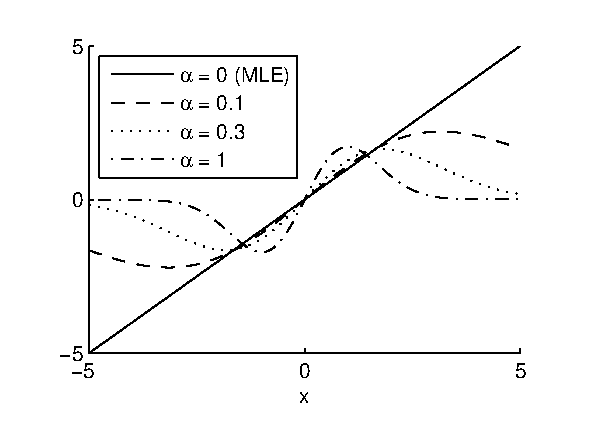
\epsfig{file=Laplace-IF-mu.eps, height=2.in} 
	&&
	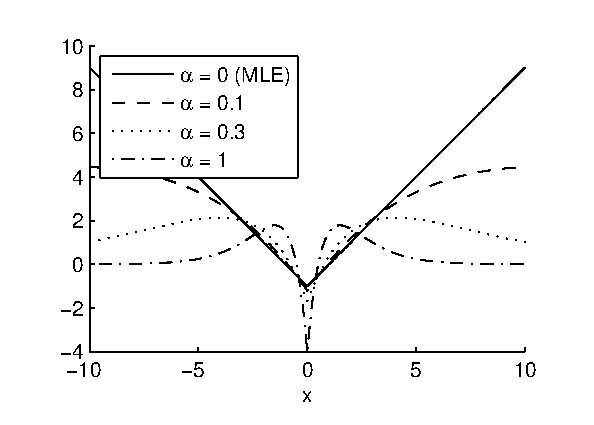
\epsfig{file=Laplace-IF-lambda.eps, height=2.in} 
	\\
	$\mathrm{IF}(x;T_{\mathfrak{R}_\alpha},\mu = 0) $ in case of known $\lambda = 1$ 
	&&
	$\mathrm{IF}(x;T_{\mathfrak{R}_\alpha},\lambda = 1)$ in case of known $\mu = 0$ 
	\\
\end{tabular}
\caption{Influence function of \mRa-estimators of parameters of Laplace distribution}
\label{fig:laplace-if}
\end{center}
%\label{fig:laplace-if}
\end{figure}

From \eqref{IF-laplace-mu} and \eqref{IF-laplace-lambda} we can see, that both influence functions are for $\alpha>0$ bounded, therefore B-robust. 

Moreover for both functions it holds that 

\begin{equation}
	\lim_{x \rightarrow \pm\infty} \mathrm{IF}(x;T_{\mathfrak{R}_\alpha},\cdot) = 0.
\end{equation}
 
\noindent Although the rejection points $\rho^*$ isn't finite, but the limits hold. We can see, that this convergence has exponential development in $\alpha$ due to the component  $e^{-\alpha x}$ in both functions. This means, that the estimator is more robust with higher value of $\alpha$. This can be also seen in the figure \ref{fig:laplace-if}, where the influence functions for both estimated parameters are shown separately for various $\alpha$.  We can see that maximum likelihood estimator $(\alpha = 0)$ isn't bounded and that the functions approach 0 faster with increasing $|x|$ for higher values of $\alpha$.

\subsection{Exponential distribution} 
Here we use \mRa-estimators to estimate parameter $\theta = (\mu,\lambda)$ of exponential distribution with probability density function 
\begin{equation}
	p_\theta = \frac{1}{\lambda} e^{-\frac{x-\mu}{\lambda}}, \qquad \mu\in \mathbb{R},\, \lambda>0, \, x\geq\mu.
\end{equation}
\noindent Exponential density's form is very similar to that of Laplace density. Below we will see, that even formulas for \mRa-estimators are very similar in both models. For $\alpha = 0$ we get \mRa-estimator in the form
\begin{align}
	\hat{\theta}_{\mathfrak{R}_0,n} & =  \arg \max_{\theta \in \Theta} \frac{1}{n} \sum^n_{i=1} \ln \left[ \frac{1}{\lambda}\exp \left[-\frac{x_i-\mu}{\lambda} \right] \right] \nonumber \\
	& =  \arg \max_{\theta \in \Theta} \left[ \ln \frac{1}{\lambda} - \frac{1}{n} \sum^n_{i=1} \frac{x_i-\mu}{\lambda} \right].
\end{align}

\noindent Condition \ref{eq:betaCond} holds again for all  $\beta>0$, therefore we can write \mRa-estimator for exponential family for $\alpha>0$ as
\begin{equation}
	\hat{\theta}_{\mathfrak{R}_\alpha,n} = \arg \max_{\theta \in \Theta} \lambda^{-\frac{\alpha}{1+\alpha}} \frac{1}{n}\sum_{i=1}^n \exp \left[-\alpha\frac{x_i-\mu}{\lambda} \right].
	\label{renyi-formula-exponential}
\end{equation}

We can see, that the difference to \eqref{renyi-formula-laplace} is only in the use of absolute value in Laplace model.

For  the estimator of location $\hat{\theta} = \mu$ in case of known $\lambda$, the influence function is the same as in the Laplace family $\eqref{IF-laplace-mu}$, therefore it holds

\begin{equation}
	\mathrm{IF}(x;T_{\mathfrak{R}_\alpha},\mu) = (1+\alpha )^{\frac{3}{2}} (x-\mu )  e^{-\frac{\alpha}{2} (x-\mu )^2}. % IF(x,mu)
	\label{IF-exponential-mu}
\end{equation}
If we estimate parameter of scale $\hat{\theta} = \lambda$ in case of known $ \mu $, we get formula
\begin{equation}
	\mathrm{IF}(x;T_{\mathfrak{R}_\alpha},\lambda) =	(1+\alpha )^2 \left( - \lambda +(1+ \alpha)(x-\mu)\right) e^{-\frac{\alpha (x-\mu)}{\lambda }}. % IF(x,lambda),
	\label{IF-exponential-lambda}
\end{equation}

\begin{figure}[htb]
\begin{center}
\begin{tabular}{c c c}
	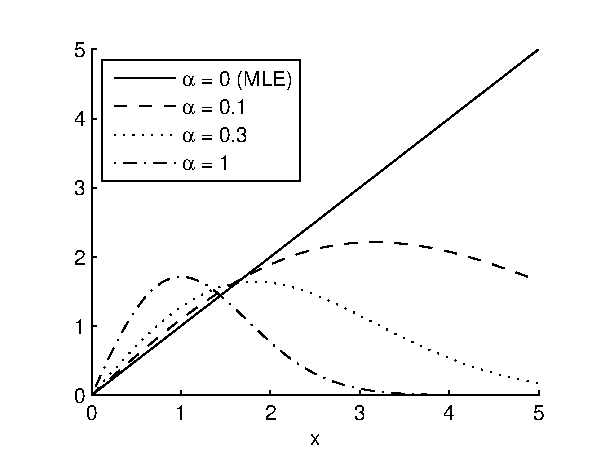
\epsfig{file=Exp-IF-mu.eps, height=2.1in} 
	&&
	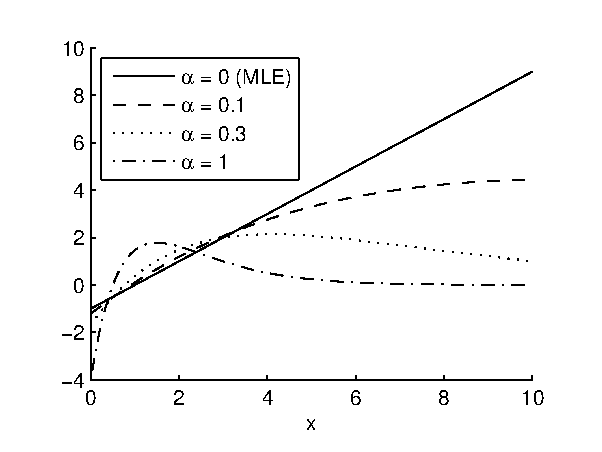
\epsfig{file=Exp-IF-lambda.eps, height=2.1in} 
	\\
	$\mathrm{IF}(x;T_{\mathfrak{R}_\alpha},\mu = 0) $ in case of known $\lambda = 1$
	&&
	$\mathrm{IF}(x;T_{\mathfrak{R}_\alpha},\lambda = 1)$ in case of known $\mu = 0$
	\\
\end{tabular}
\caption{Influence function of \mRa-estimators of parameters of exponential distribution}
\label{fig-exp-if}
\end{center}
\end{figure}

\noindent We can see from \eqref{IF-exponential-mu} and \eqref{IF-exponential-lambda} that for both functions it holds, that

\begin{equation}
	\lim_{x \rightarrow \pm\infty} \mathrm{IF}(x;T_{\mathfrak{R}_\alpha},\cdot) = 0,
\end{equation}
therefore outliers will be partially ignored due to the convergence of influence functions to 0. Again it holds, that the convergence is faster with greater $\alpha$, which can be seen in figure \ref{fig-exp-if}, as well as the fact, that the functions are bounded for all $\alpha >0$.

\subsection{Cauchy distribution} 
In this section we derive formulas for \mRa-estimators for Cauchy distribution with parameter $\theta = (\mu,\sigma)$ and probability density function
\begin{equation}
	p_\theta = \frac{1}{\pi\sigma} \left( 1 + \left( \frac{x-\mu}{\sigma} \right)^2 \right)^{-1}, \qquad \mu\in \mathbb{R},\, \sigma>0.
\end{equation}
Min $\mathfrak{R}_\alpha$-estimator for $\alpha=0$  coincides with the maximum likelihood estimator
\begin{align}
	\hat{\theta}_{\mathfrak{R}_0,n} & = \arg \max_{\theta \in \Theta} \frac{1}{n} \sum^n_{i=1} \ln \left[  \frac{1}{\pi\sigma} \left( 1 + \left( \frac{x_i-\mu}{\sigma} \right)^2 \right)^{-1}   \right] \nonumber \\
	& =  \arg \max_{\theta \in \Theta} \left[ -\ln \pi\sigma - \frac{1}{n} \sum^n_{i=1} \ln \left[ 1 + \left( \frac{x_i-\mu}{\sigma} \right)^2 \right] \right].
\end{align}
Condition \ref{eq:betaCond} holds as in previous cases for all $\beta>0$. For $\alpha>0$ we get \mRa-estimator \eqref{eq:renEstimator} in Cauchy model in the form 

\begin{equation}
	\hat{\theta}_{\mathfrak{R}_\alpha,n} = \arg \max_{\theta \in \Theta} \left[ \sigma^{-\frac{\alpha}{1+\alpha}} \frac{1}{n} \sum_{i=1}^n \left( 1 + \left( \frac{x_i-\mu}{\sigma} \right)^2 \right)^{-\alpha} \right].
	\label{renyi-formula-cauchy}
\end{equation}

We were able to calculate influence function \eqref{eq:IF} for \mRa-estimator only for parameter of location $\theta = \mu$. Assuming known scale $\sigma$, we get function

\begin{equation}
	\mathrm{IF}(x;T_{\mathfrak{R}_\alpha},\mu) = \sqrt{\pi}\frac{\Gamma\left( 3 + \alpha \right)}{\Gamma\left( \frac{3}{2} + \alpha \right)} \left( \frac{\sigma^2}{\sigma^2 + (x-\mu)^2}\right)^{1+\alpha}(x-\mu).
	\label{IF-cauchy-mu}
\end{equation}

We can see from  \eqref{IF-cauchy-mu} and figure \ref{fig:cauchy-if}, that the influence function is bounded for all $\alpha>0$. Rejection point $\rho^*$ is not finite, but for $\alpha>0$ at least the limit 
\begin{equation}
	\lim_{x \rightarrow \pm\infty} \mathrm{IF}(x;T_{\mathfrak{R}_\alpha},\mu) = 0.
\end{equation}
holds.
\begin{figure}[htb]
\begin{center}
\begin{tabular}{c}
	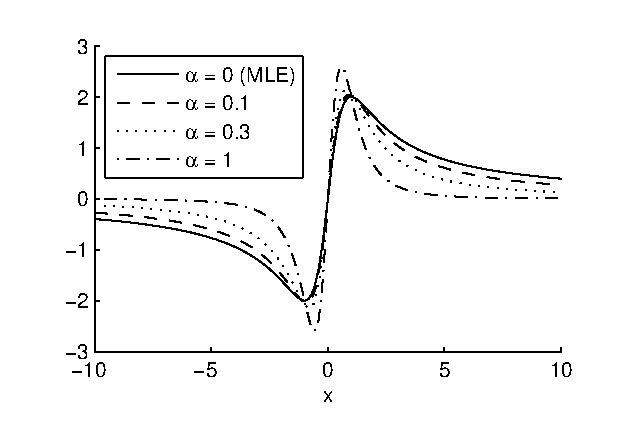
\epsfig{file=Cauchy-IF-mu.eps, height=2.6in} \\
	$\mathrm{IF}(x;T_{\mathfrak{R}_\alpha},\mu = 0) $ in case of known $\sigma = 1$
\end{tabular}
\caption{Influence function of \mRa-estimators of parameter of Cauchy distribution}
\label{fig:cauchy-if}
\end{center}
\end{figure}

According to \eqref{eq:IF} we could find the formula for estimator of scale $\theta = \sigma$ in case of known location $\mu$. The following result is obtained via computation in software tool \texttt{Wolfram Mathematica}

\begin{eqnarray}
\mathrm{IF}(x;T_{\mathfrak{R}_\alpha},\sigma) &=& -\left[4 \sqrt{\pi } (1+\alpha )^2 \sigma ^{2+\alpha } \left(\frac{\sigma }{(x-\mu )^2+\sigma ^2}\right)^{\alpha} \right. \nonumber\\
&&\left(\frac{1}{\sigma }+\frac{\alpha  \left(\frac{1}{\sigma }\right)^{\alpha } \sigma ^{-1+\alpha }}{1+\alpha }-\frac{2 \sigma }{(x-\mu )^2+\sigma ^2}\right) \left. \cos[\pi  \alpha ] \Gamma[\alpha ] \Gamma[1+\alpha ]  \frac{}{} \right] / \nonumber \\ %prázdný zlomek je tam kvůli roztažení koncové závorky
&&\left(4^{1-\alpha } \sqrt{\pi } \left(\frac{1}{\sigma }\right)^{\alpha } \sigma ^{\alpha } \left(-1+\alpha  \left(-1+\alpha  \left(-2+\left(\frac{1}{\sigma }\right)^{\alpha } \sigma ^{\alpha }\right)\right)\right) \right.\nonumber \\ 
&&\left. \cos[\pi  \alpha ] \Gamma[1+2 \alpha ]+1/(3 (3+4 \alpha  (2+\alpha )))\right. \nonumber \\
&& 8 \pi  (1+\alpha ) \left(-1+\alpha  (1+\alpha )^2\right) \Gamma[\alpha ] \nonumber \\
&& \left(6 (1+\alpha ) ^r_2\mathrm{F}_1\left[\frac{1}{2},2,\frac{1}{2}-\alpha ,1\right]-4^{-\alpha } \Gamma[4+2 \alpha ] \right. \nonumber \\
&& \left. \left. ^r_2\mathrm{F}_1\left[\frac{1}{2}+\alpha ,1+\alpha ,-\frac{1}{2}+\alpha ,1\right]\right)\right),
\end{eqnarray}

\noindent where $^r_2\mathrm{F}_1[a,b;c;z]$ is regularized hypergeometric function

\begin{equation}
	^r_2\mathrm{F}_1[a,b;c;z] = {\frac{1}{\Gamma[c]}} {_2\mathrm{F}_1}[a,b;c;z],
\end{equation}
where hypergeometric function is defined as
\begin{equation}
	{_2\mathrm{F}_1}[a,b;c;z]=\sum _{n=0}^{\infty } \frac{(a)_n (b)_n z^n}{ (c)_n n!}, \qquad |z|<1, \, \text{ nebo } \, (|z|=1\l  \,\text{a} \,  c>a+b),
\end{equation}

\noindent where $(a)_n$ is Pochhammer symbol defined as

\begin{equation}
(a)_n=\prod _{k=0}^{n-1} (a+k), \qquad n \in \mathbb{N}.
\end{equation}

\noindent Because of the definition of hypergeometric function this influence function doesn't make sense, because from definition constraints we get $\frac{1}{2}+\alpha  + 1+\alpha < -\frac{1}{2}+\alpha $, thus  $\alpha < -2$, which contradicts the constraint  $\alpha>0$ from theorem \ref{eq:betaCond}. 

\subsection{Weibull distribution} 

Last distribution where we got some results was three-parameter Weibull with $\theta = (\mu,\lambda,k)$ and probability density
\begin{equation}
	p_\theta =  \frac{k}{\lambda} \left( \frac{x-\mu}{\lambda} \right)^{k-1} \exp \left[ -\left( \frac{x-\mu}{\lambda} \right)^k \right], \qquad \mu \in \mathbb{R}, \, \lambda>0, \, k>0, \, x \geq \mu.
\end{equation}

\noindent For $\alpha = 0$ is \mRa-estimator equal to

\begin{align}
	\hat{\theta}_{\mathfrak{R}_0,n} & = \arg \max_{\theta \in \Theta} \frac{1}{n} \sum^n_{i=1} \ln \left[ \frac{k}{\lambda} \left( \frac{x_i-\mu}{\lambda} \right)^{k-1} 
	\exp \left[ -\left( \frac{x_i-\mu}{\lambda} \right)^k \right]\right] \nonumber \\
	&=\arg \max_{\theta \in \Theta}\left[ \ln \frac{k}{\lambda} + \frac{k-1}{n} \sum^n_{i=1} \ln \left[  \frac{x_i-\mu}{\lambda} \right] - 
	\frac{1}{n} \sum^n_{i=1} \left(  \frac{x_i-\mu}{\lambda} \right)^k \right].
\end{align}

\noindent Condition \ref{eq:betaCond} holds again for all $\beta>0$. For $\alpha>0$ we get the \mRa-estimator \eqref{eq:renEstimator} in the form

\begin{eqnarray}
	\hat{\theta}_{\mathfrak{R}_\alpha,n} & = & \arg \max_{\theta \in \Theta} \left( \frac{k}{\lambda} \right)^\frac{\alpha}{1+\alpha} (1+\alpha)^{\frac{\alpha}{1+\alpha}\frac{1+\alpha+k}{k}} 
	\Gamma\left(\frac{1+\alpha+k}{k}\right)^{-\frac{\alpha}{1+\alpha}} \nonumber \\
	&& \frac{1}{n}\sum_{i=1}^n \left( \frac{x_i-\mu}{\lambda}\right)^{\alpha(k-1)} \exp\left[-\alpha \left(\frac{x_i-\mu}{\lambda}\right)^k\right].
\end{eqnarray}

\noindent Because of use of $\Gamma$-function we get additional constraint  $1+\alpha+k>0$, thus $\alpha + k > -1$. This constraint is always satisfied, because both members on the left side are positive.

Influence function $\eqref{eq:IF}$ for estimator of location $\hat{\theta} = \mu$ in case of known $\lambda, k $  can be written as

\begin{equation}
	\mathrm{IF}(x;T_{\mathfrak{R}_\alpha},\mu) = \frac{(1+\alpha )^{\frac{-2-\alpha +k (3+\alpha )}{k}} \lambda \left(1+k \left(-1+\left(\frac{x-\mu }{\lambda }\right)^k\right)\right) 
	 \left(\frac{x-\mu }{\lambda }\right)^{\alpha k-\alpha-1}\exp \left[-\alpha\left(\frac{x-\mu }{\lambda }\right)^k\right]}
	 {(-1+k) (-1+k+k \alpha ) \Gamma\left[\frac{-2+k+(-1+k) \alpha }{k}\right]}.
	\label{IF-weibull-mu}
\end{equation}

\noindent From the use of $\Gamma$-function we get constraint $k > 1 + \frac{1}{1+\alpha}$, thus $(\forall \alpha> 0) (k > 1)$. Because of the exponential member, for $\alpha > 0$ we again get the limit

\begin{equation}
	\lim_{x \rightarrow \pm\infty} \mathrm{IF}(x;T_{\mathfrak{R}_\alpha},\mu) = 0.
\end{equation}

\begin{figure}[!htb]
\begin{center}
\begin{tabular}{cc}
	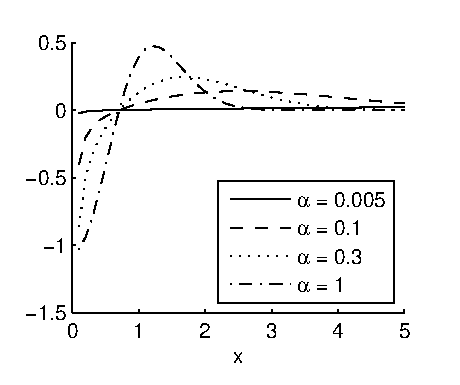
\epsfig{file=Weib-IF-mu.eps, height=2.2in} & 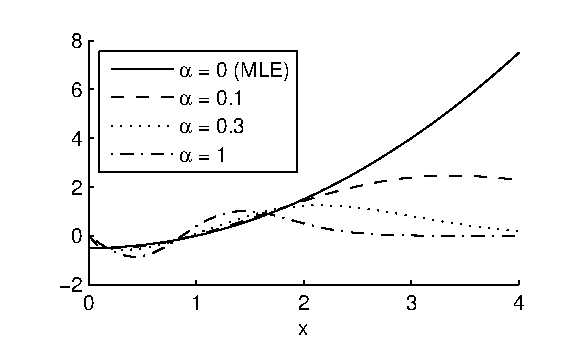
\epsfig{file=Weib-IF-lambda.eps, width=3.2in}
	\\	
	$\mathrm{IF}(x;T_{\mathfrak{R}_\alpha},\mu = 0) $, in case of known $\lambda = 1, \: k = 2$ & $\mathrm{IF}(x;T_{\mathfrak{R}_\alpha},\lambda = 1) $, in case of known $\mu = 0, \: k = 2$
\end{tabular}
\caption{Influence function of \mRa-estimators of $\mu$ and $\lambda$ in Weibull distribution}
\label{figJK:weibull-if}
\end{center}
\end{figure}

\noindent In the figure \ref{figJK:weibull-if} we can see, that influence function is again bounded. There is not function for $\alpha = 0$ in the left figure, because for $k=2$ we have to use $\alpha >0$.
For the estimation of sccale $\theta = \lambda$ in case of known $\mu, k$, the influence function can be written as

\begin{equation}
	\mathrm{IF}(x;T_{\mathfrak{R}_\alpha},\lambda) = \frac{(1+\alpha )^{2+\alpha -\frac{\alpha }{k}} \lambda  \left(\alpha +k (1+\alpha ) \left(-1+\left(\frac{x-\mu }{\lambda }\right)^k\right)\right)
	\left(\frac{x-\mu}{\lambda}\right)^{\alpha k-\alpha} \exp \left[-\alpha\left(\frac{x-\mu}{\lambda}\right)^k\right]}
	{k^2 \Gamma\left[2+\alpha -\frac{\alpha }{k}\right]}.
	\label{IF-weibull-lambda}
\end{equation}

\noindent From the use of $\Gamma$-function we get additional constraint $k>\frac{\alpha}{2+\alpha}$. Function for $\alpha > 0$ and $x\rightarrow \pm \infty$ converges to $0$ and it is bounded, which we can see on figure \ref{figJK:weibull-if}. For the commputation of influence function for the estimated parameter $\hat{\theta} = k$ \texttt{Wolfram Mathematica} to the result of

\begin{eqnarray}
	\mathrm{IF}(x;T_{\mathfrak{R}_\alpha},k)& = &\left(k^2 (1+\alpha )^{2+\alpha -\frac{\alpha }{k}} \left(e^{-\left(\frac{x-\mu }{\lambda }\right)^k} \left(\frac{x-\mu }{\lambda }\right)^{-1+k}\right)^{\alpha } \right. \nonumber \\
	&& \left(\alpha  \text{ln}[1+\alpha ]+k \left(1-k (1+\alpha ) \left(-1+\left(\frac{x-\mu }{\lambda }\right)^k\right)\right.\right. \nonumber \\
	&& \left.\left.\left.\left.\text{ln}\left[\frac{x-\mu }{\lambda }\right]\right)-\alpha  \psi\left[0,1+\alpha -\frac{\alpha }{k}\right]\right)\right)\right/ \nonumber \\
	&& \left(\Gamma\left[1+\alpha -\frac{\alpha }{k}\right] (k (k+\ln[1+\alpha ] \right.  \\
	&& (-2 k+2 \alpha +(k+(-1+k) \alpha ) \ln[1+\alpha ]))-2 k (-k+\alpha + \nonumber \\
	&& (k+(-1+k) \alpha )\ln[1+\alpha ]) \psi\left[0,1+\alpha -\frac{\alpha }{k}\right]+k (k+(-1+k) \alpha ) \nonumber \\
	&& \left.\left.\psi\left[0,1+\alpha -\frac{\alpha }{k}\right]^2+\left(k^2+(-1+k) k \alpha +\alpha ^2\right) \psi\left[1,1+\alpha -\frac{\alpha }{k}\right]\right)\right), \nonumber
	\label{IF-weibull-k}
\end{eqnarray}

\noindent where $\psi(n,z)$ is $(n+1)^\text{th}$ differentiation of logarithm of $\Gamma(z)$, thus

\begin{equation}
	\psi(n,z) = \frac{\mathrm{d}^{n+1}}{\mathrm{d}z^{n+1}} \ln \Gamma(z).
\end{equation}

\noindent Because of the use of $\Gamma$-function we need $k > \frac{\alpha}{1+\alpha}$. Function is bounded for $\alpha>0$ and for $x$ going to infinity, the function converges to 0.

\begin{figure}[htb]
\begin{center}
\begin{tabular}{cc}	
	\multicolumn{2}{c}{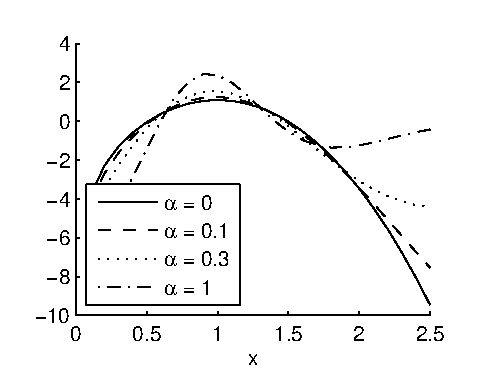
\epsfig{file=Weib-IF-k.eps, height=2.5in}}
	\\
	\multicolumn{2}{c}{$\mathrm{IF}(x;T_{\mathfrak{R}_\alpha},k = 2) $, in case of known $\mu = 0, \: \lambda = 1$}
\end{tabular}
\caption{Influence function for \mRa-estimator of $k$ in Weibull distribution}
\label{figJK:weibull2-if}
\end{center}
\end{figure}



 


